\documentclass{article}

\usepackage[english]{babel}
\usepackage[utf8x]{inputenc}
\usepackage{amsmath}
\usepackage{amsthm}
\usepackage{graphicx}
\usepackage[colorinlistoftodos]{todonotes}
\usepackage{float}

\title{CS 419 Term Project}
\author{\emph{Anthony Tyrrell}}

\begin{document}
\maketitle
\tableofcontents
\newpage
\section{Explanation and Motives}

Over the course of this class we (the undergraduates) completed homework's on the topics of Scan Line conversion, Matrix transformations, and Shading. Although these assignments consisted of technical work, the overall concept of this course was a conceptual look at the Rendering Equation. When analyzing the rendering equation, you break down all of its components into smaller modules. As a result your render equation has view ports, geometry, shading and lighting to name a few. Once this separation in components became clear to me, I gained a lot of interest in Ray Trace engines. Since the undergraduates did not complete the Ray Trace engine, I figured it would be a good topic to cover for the final project.

Ray Trace engines are the epitome of visual realistic image rendering. While they still give the effect of a “CG” look, they provided a higher level of detail that scan line conversion could ever hope to. Ray Trace engines are also ripe for parallelism, making them a computationally effective way to render complex images. 

\section{Engine Decomposition}
\subsection{
Modules
}
\begin{itemize}
  \item Lighting - Defined in Lighting.cpp and Lighting.h. 
  
Contains custom class Light that holds information such as light color, position, direction and intensity.
  
  \item Geometry - Defined in Sphere.cpp and Sphere.h

Contains custom classes for objects, overloads include triangle and sphere objects. 
Rays -Defined in Ray.cpp and Ray.h

Contains custom class Ray(). Also contains functions GetNearestHit() that finds object intersections based on object location.
  
  \item Colors - Defined in Color.cpp and Color.h
  
  Contains custom class Color() and class functionalities. The goal of this was to make colors uniformly represented throughout the Ray Trace Engine.
  
  \item Camera - Defined in Camera.cpp and Camera.h
  
  Contains custom Camera() class. Supports Orthographic and Perspective viewing modes.


\end{itemize}
\subsection{Features}
\begin{itemize}
	\item MultiThreading - Implemented with OpenMP in Visual Studio

	Basic multithreading with inspiration from my CS475 Parallel Computing course I'm taking this term. Parallelizes the Ray Trace of the pixels.
    
	\item Hard Shadows - Implemented by calculation additional ray bounces from the object to the light source and checking object intersections.
    
    \item Specular Highlights - Specular lighting implementation, able to change colors and intensity.
\end{itemize}

All of these modules with the exception of MultiThreading are pieced together inside of the file Raytrace.cpp, which includes the functions Raytrace() and CalculateLighting(). Let’s talk about those.


\section{Code Explanation and Rendering Pseudocode}
\subsection{bool RayTrace( );}
RayTrace takes a camera, list of objects, light, ray, and number of bounces as arguments. It returns a boolean True or False, depending on whether or not the given ray intersects an object in the list. If a hit is detected, information about it will be stored in RayHitInfo. 

Once a ray hit is detected, that ray, light, and object are passed to the CalculateLighting() function, which is in charge of assigning a color to that given pixel. This is done by summing Specular, Ambient, and Diffuse lighting and assigning that to the pixel. Since these values range from 0-255, the R, G, B, and A results values are assigned to a 4 byte integer. Each value occupies 8 bits of this space.

\subsection{void CalculateLighting()}
Calculate lighting is responsible for assigning Diffuse, Specular, and Ambient lighting to a certain pixel, given it already intersects with an object. This is done in the singular bounce of a light ray to the object to speedup performance. This function is also responsible for applying shadows if they are enabled. 
\subsubsection{Diffuse/Ambient}
To calculate Diffuse lighting, we take the Dot product of the object's surface normal, with the light vector (Light->Object).This gives us the intensity of the diffuse light, so to get the color we simply multiply the object's color at this location by the diffuse intensity. Due to our lack of additional bounces, we leave the ambient lighting minimal so direct light is applied or nothing is. 
\subsubsection{Specular}

If ENABLE SPECULAR LIGHTING is defined, specular lighting is gathered by calculating vectors from the light source to the point, and the camera to the point. The dot product between these two vectors is the intensity of our specular light. This gives an effect of visual realism, and provides a visual cue for the position, color, and intensity of the light source.
\subsubsection{Shadows}
In addition to Specular Lighting, I wanted to implement some sort of more advanced feature. I figured an interesting and effective addition would be shadows.To do so, I modified CalculateLighting() to ensure that when a points color is calculated, a vector is drawn from the point to the light source. If this ray intersects any objects, you know that you are in a shadow. 

The shadows implemented are quite basic, there is no variation between soft and regular shadows, just black or not. 

\subsection{Algorithm Pseudocode}
\begin{verbatim}
objList = InitObjects();
myLight = InitLights();
myCamera = InitCamera();

for pixelX in Image.height();
	for pixelY in Image.Width();
    	ray = new Ray(pixelX,pixelY)
    	if(RayTrace(camera,ray,objlist,mylight) == True)
        	pixelColor = CalculateLighting();
        else;
        	pixelColor = BLACK
		drawPixel(pixelX,pixelY,pixelColor)
\end{verbatim}

\newpage
\section{Results}
\subsection{Rendering}


Case 1: Base render with 50 percent lighting, specular highlights and shadows disabled.
\begin{figure}[H]
  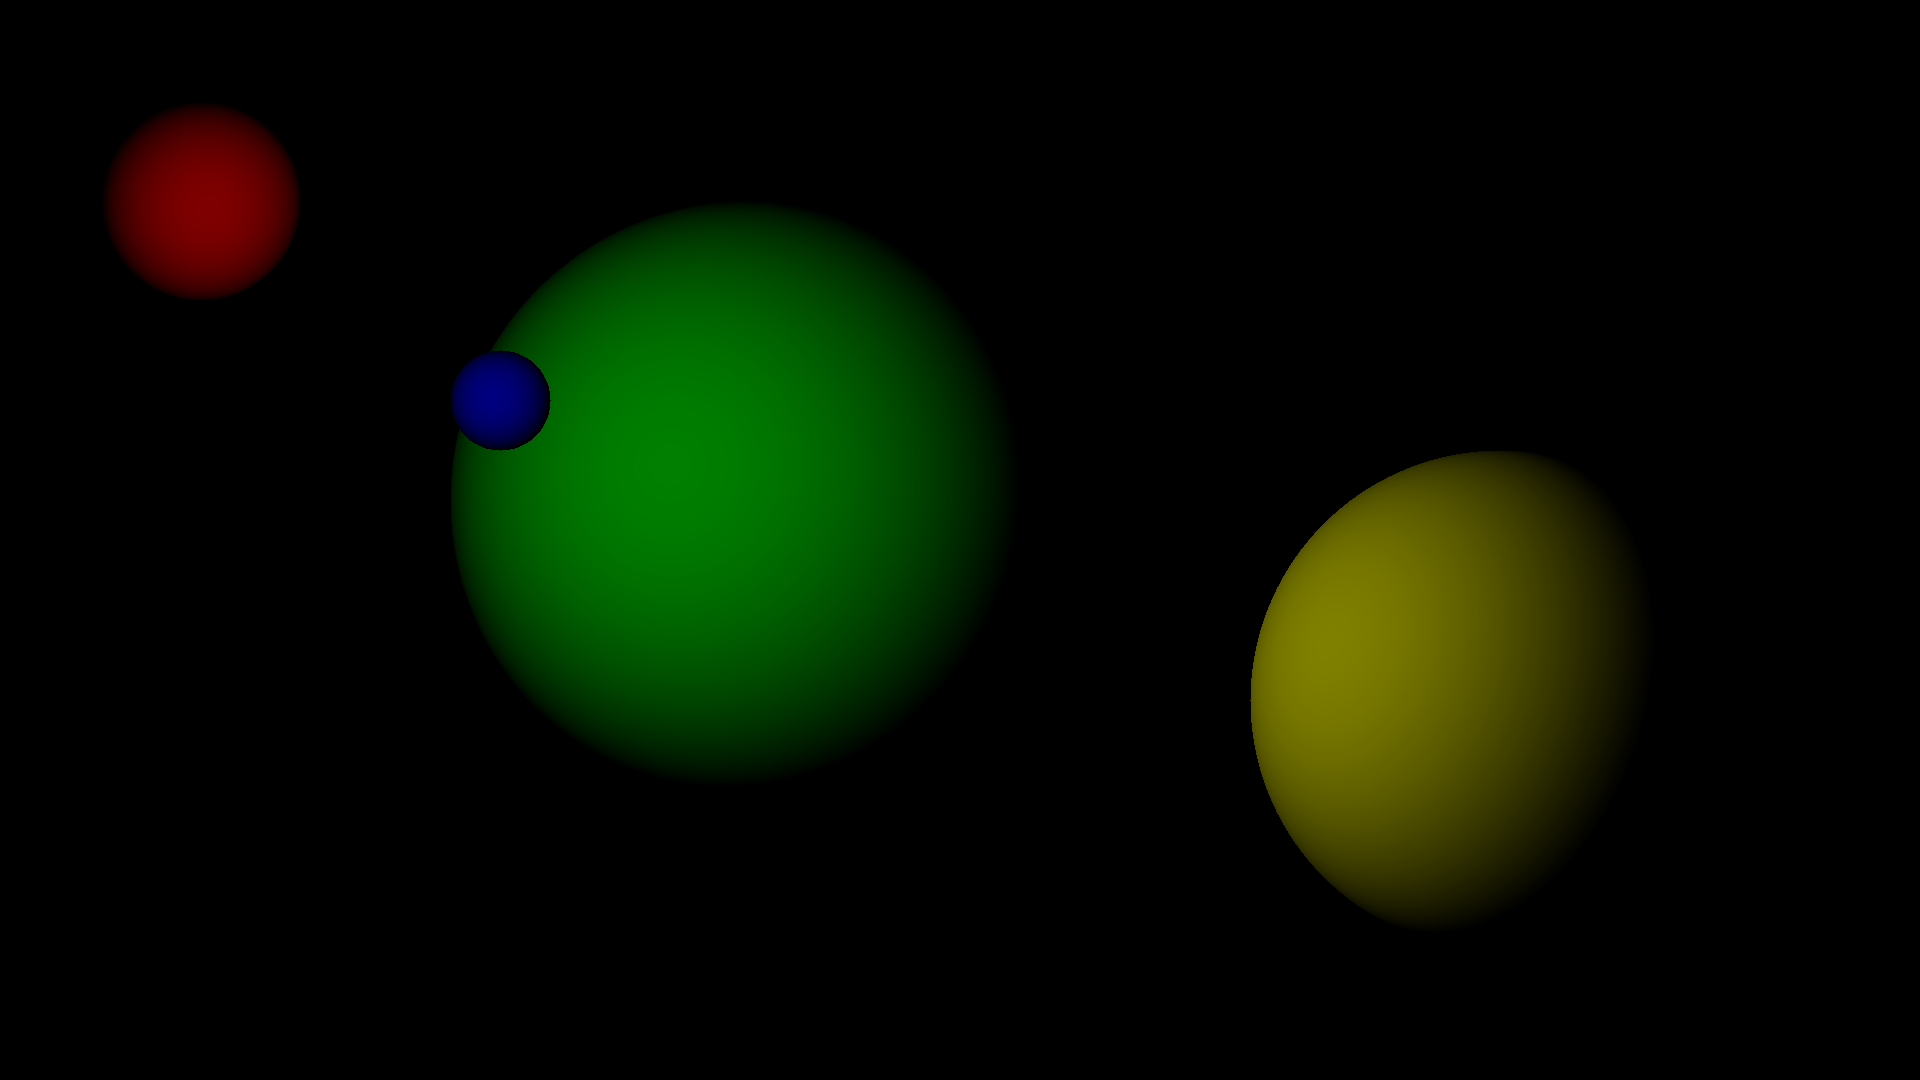
\includegraphics[width=\linewidth]{one.png}
  \caption{Scene rendered with 0.5 light intensity.}
  \label{fig:case1}
\end{figure}

Case 2: Base render full lighting. Specular highlights and shadows disabled.
\begin{figure}[H]
  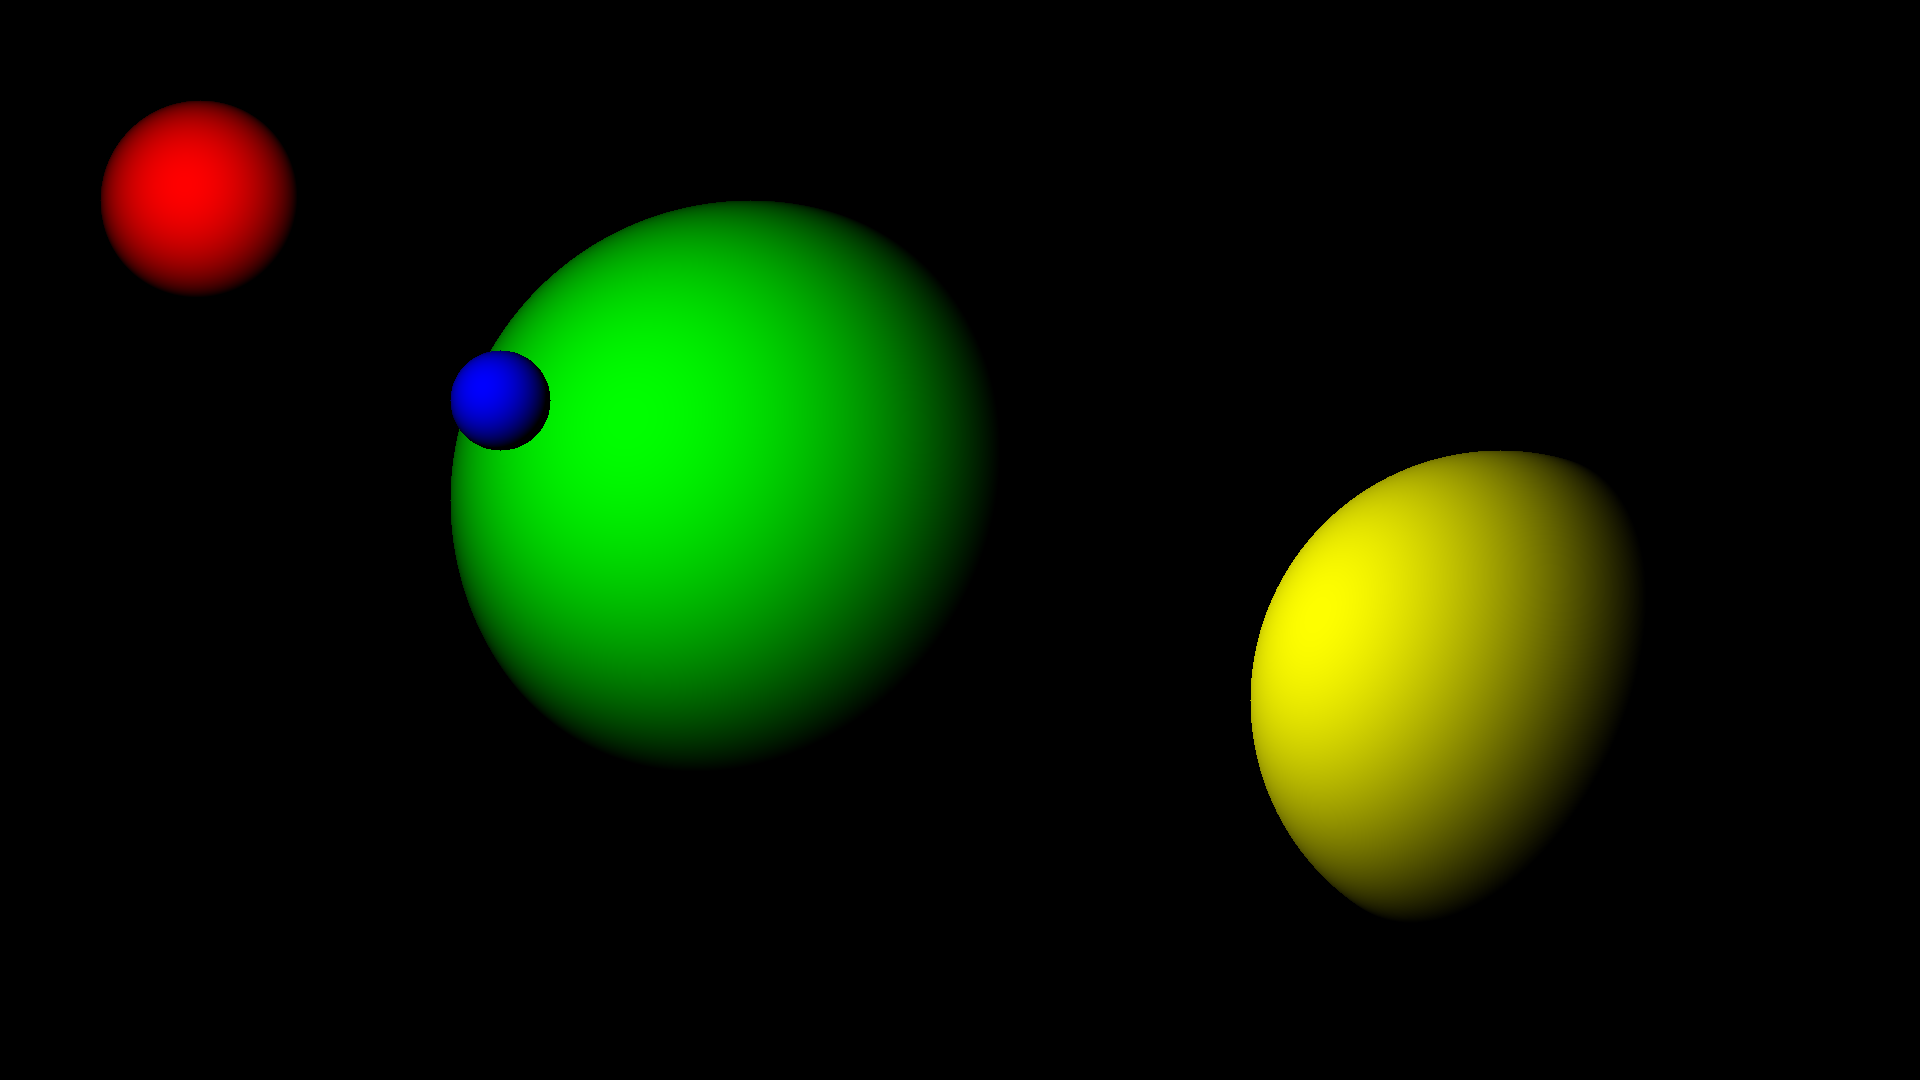
\includegraphics[width=\linewidth]{two.png}
  \caption{Scene rendered with 1.0 light intensity.}
  \label{fig:case2}
\end{figure}

Case 3: Base render with Specular Highlights enabled and Shadows disabled.
\begin{figure}[H]
  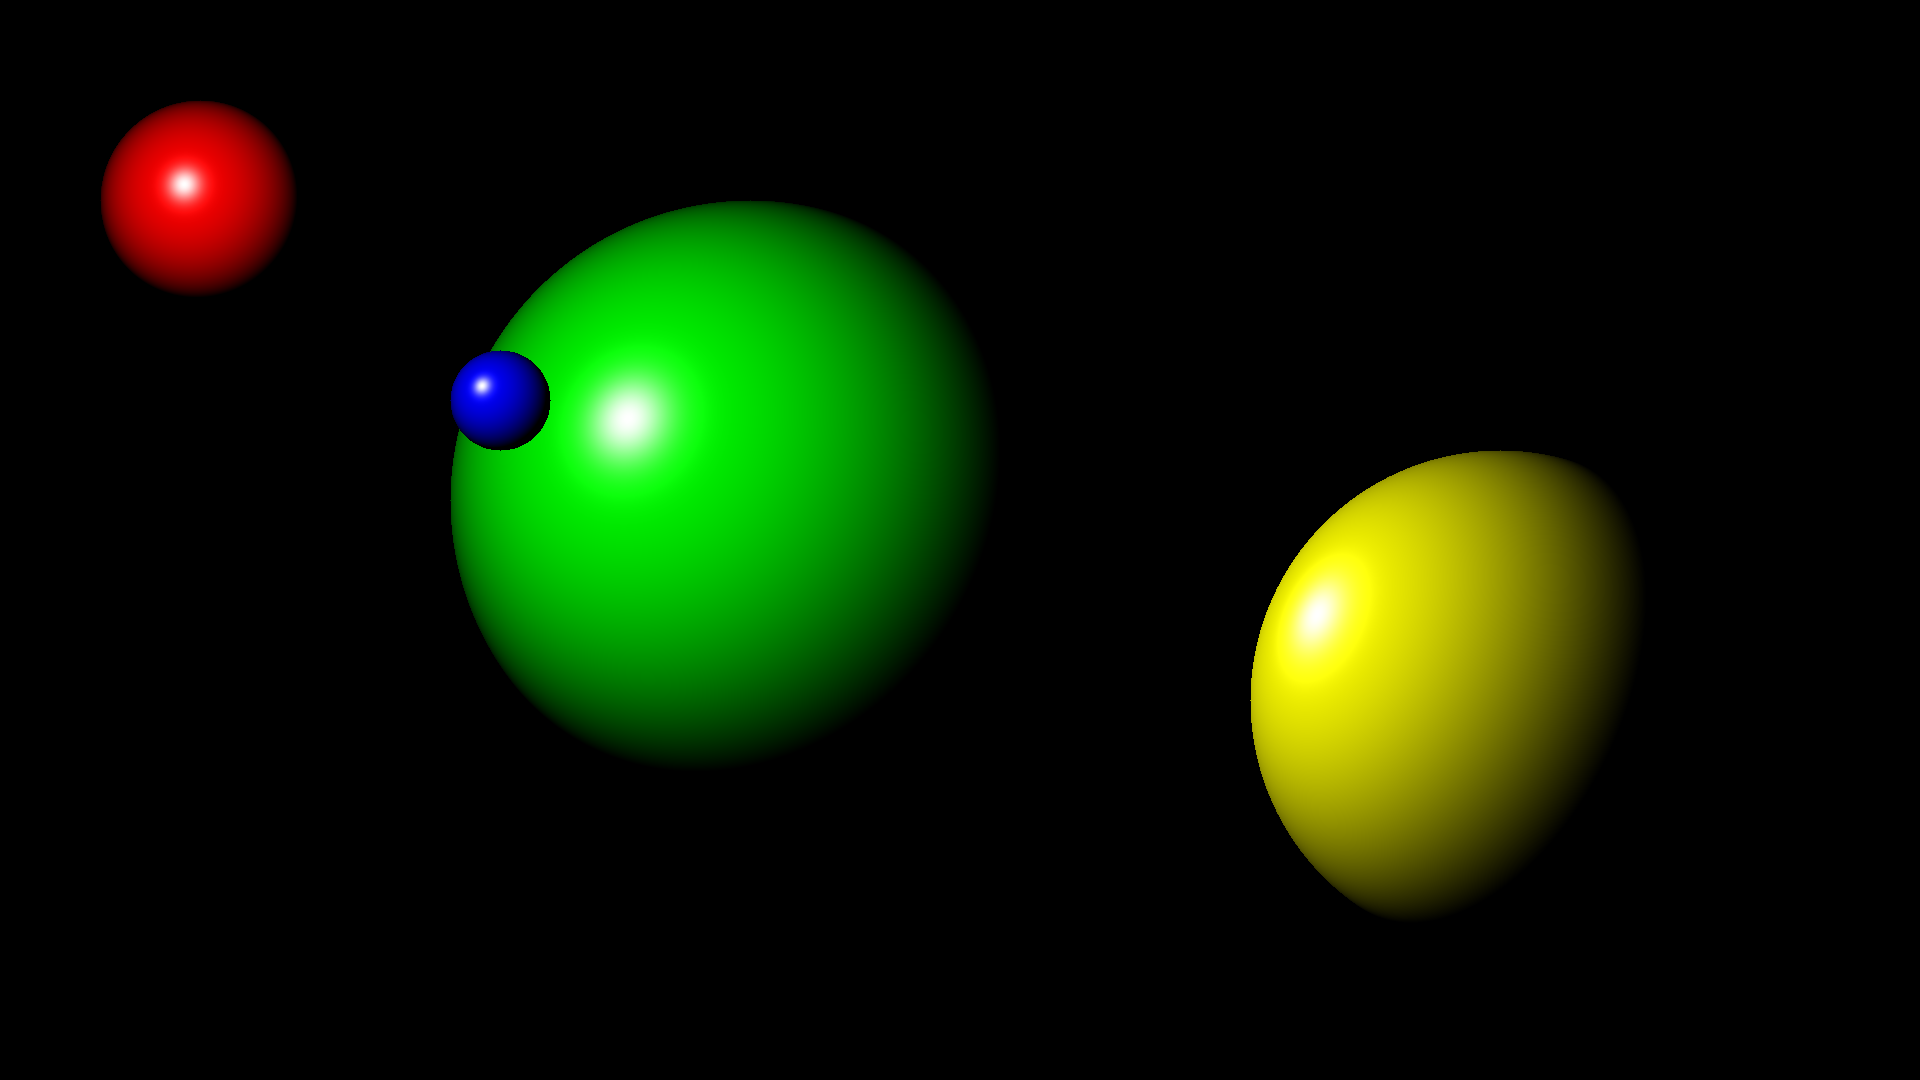
\includegraphics[width=\linewidth]{three.png}
  \caption{Scene rendered with Specular Highlights.}
  \label{fig:case3}
\end{figure}


Case 4: Base render with Specular Highlights and Shadows enabled.
\begin{figure}[H]
  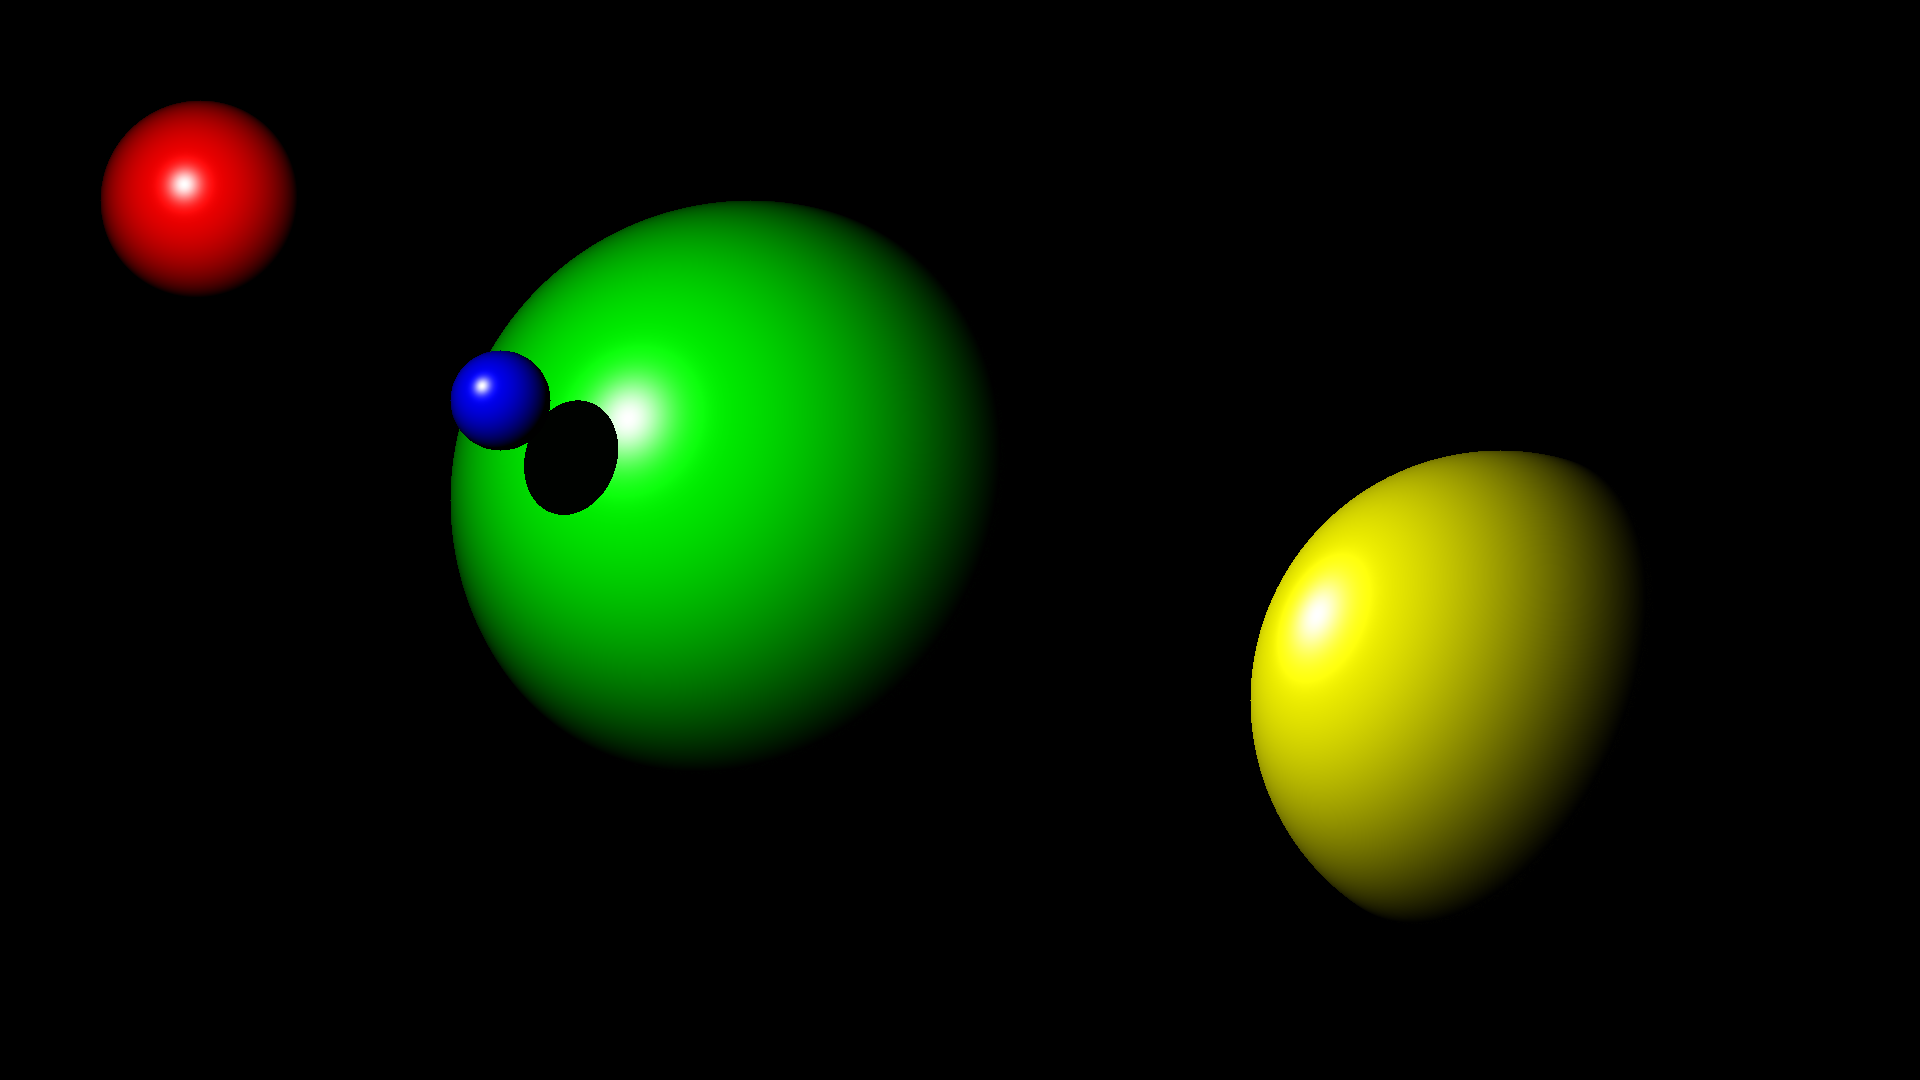
\includegraphics[width=\linewidth]{four.png}
  \caption{Scene rendered with Specular Highlights and shadows.}
  \label{fig:case4}
\end{figure}

Case 5: Base render with Specular Highlights and Shadows enabled. A white plane is drawn in the background to emphasize shadows.
\begin{figure}[H]
  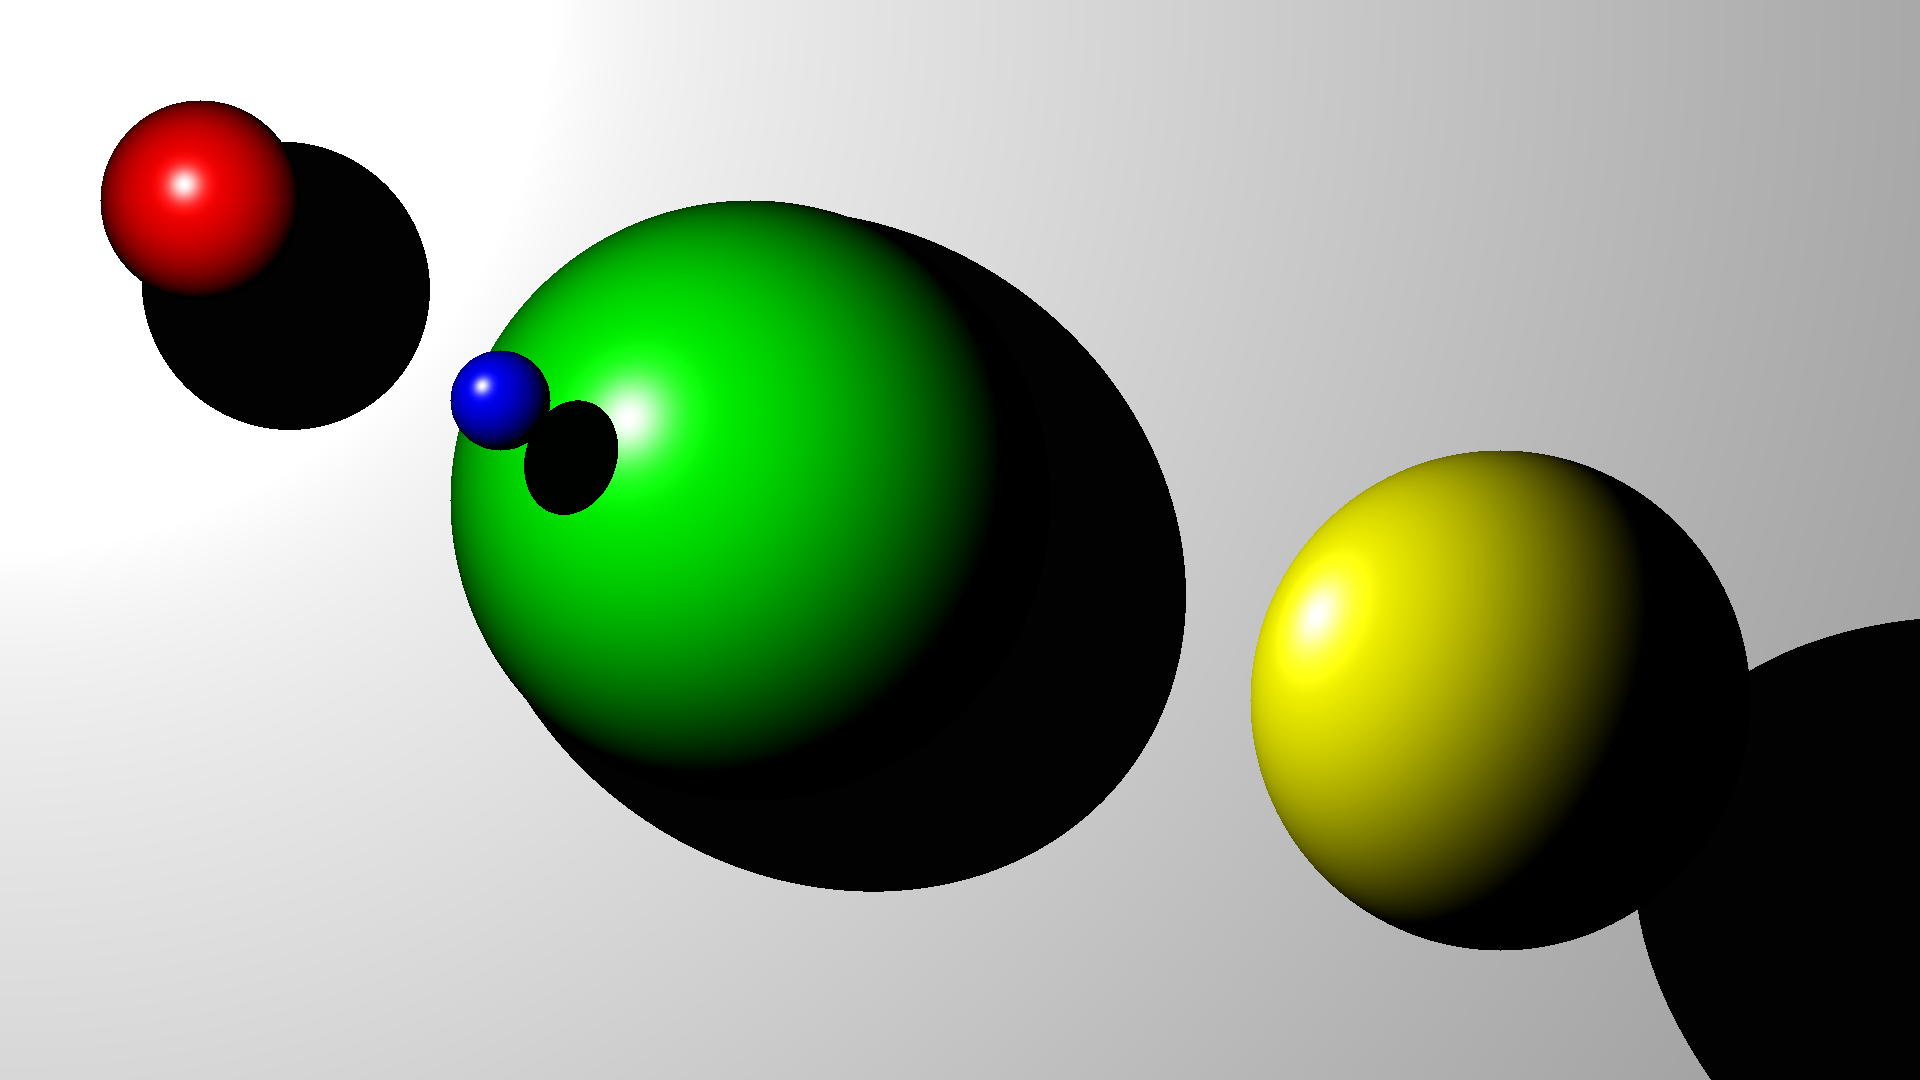
\includegraphics[width=\linewidth]{five.png}
  \caption{Scene rendered with Specular Highlights and shadows.}
  \label{fig:case5}
\end{figure}

Case 6: Base render with Specular Highlight and Shadows enabled. The light position has been shifted to show the dynamic rendering of shadows and specular lighting.
\begin{figure}[!htb]
  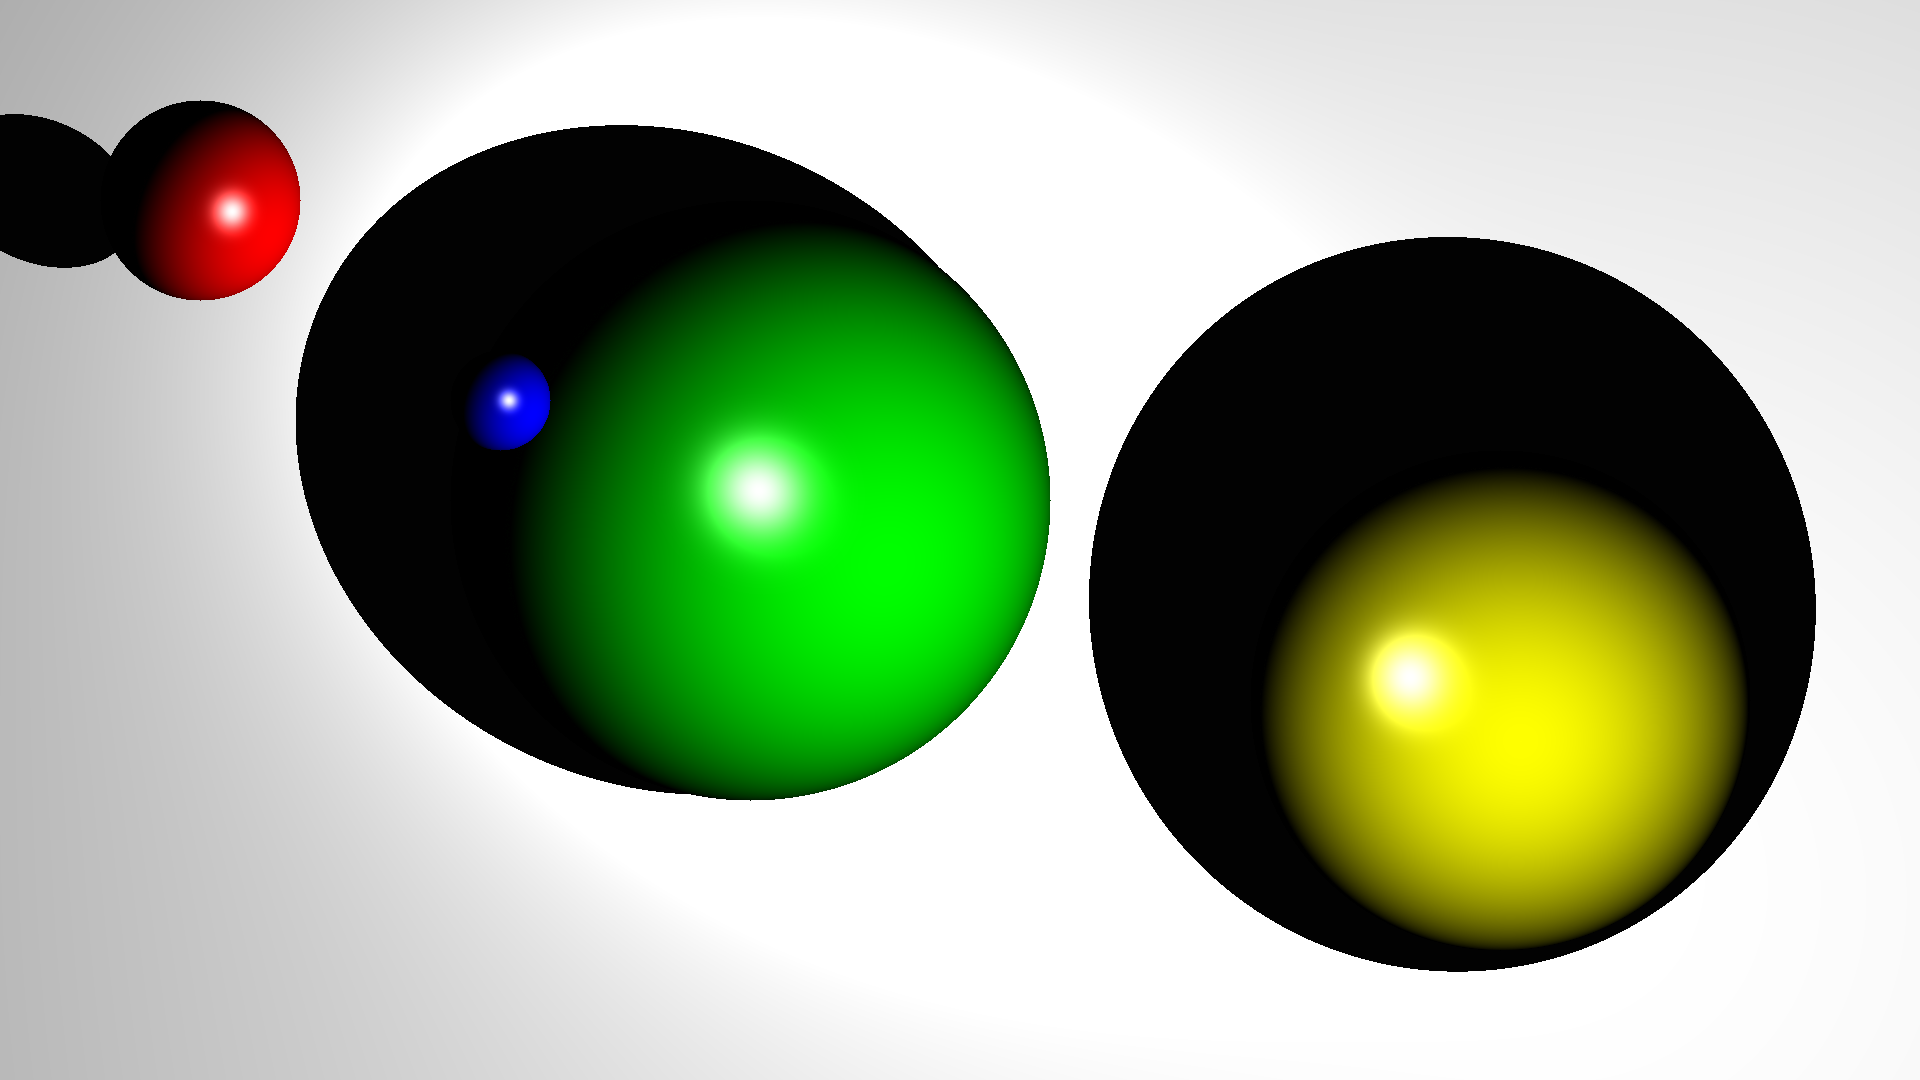
\includegraphics[width=\linewidth]{six.png}
  \caption{Scene rendered with a changing light source.}
  \label{fig:case6}
\end{figure}

\newpage
\subsection{Performance}
When analyzing the run times of the test cases, it becomes clear that the more features involved in the scene the longer it takes to render. This was very obvious for cases 5 and 6, where the white backdrop forced all of the objects to cast shadows. Section 5 talks about ways that the performance of shadows could be increased.

The table below shows a comparison of the test case run times. You can see that a few small shadows impacts run time by a few seconds, but calculating shadows for multiple objects can be very time consuming. 
\begin{figure}[H]
  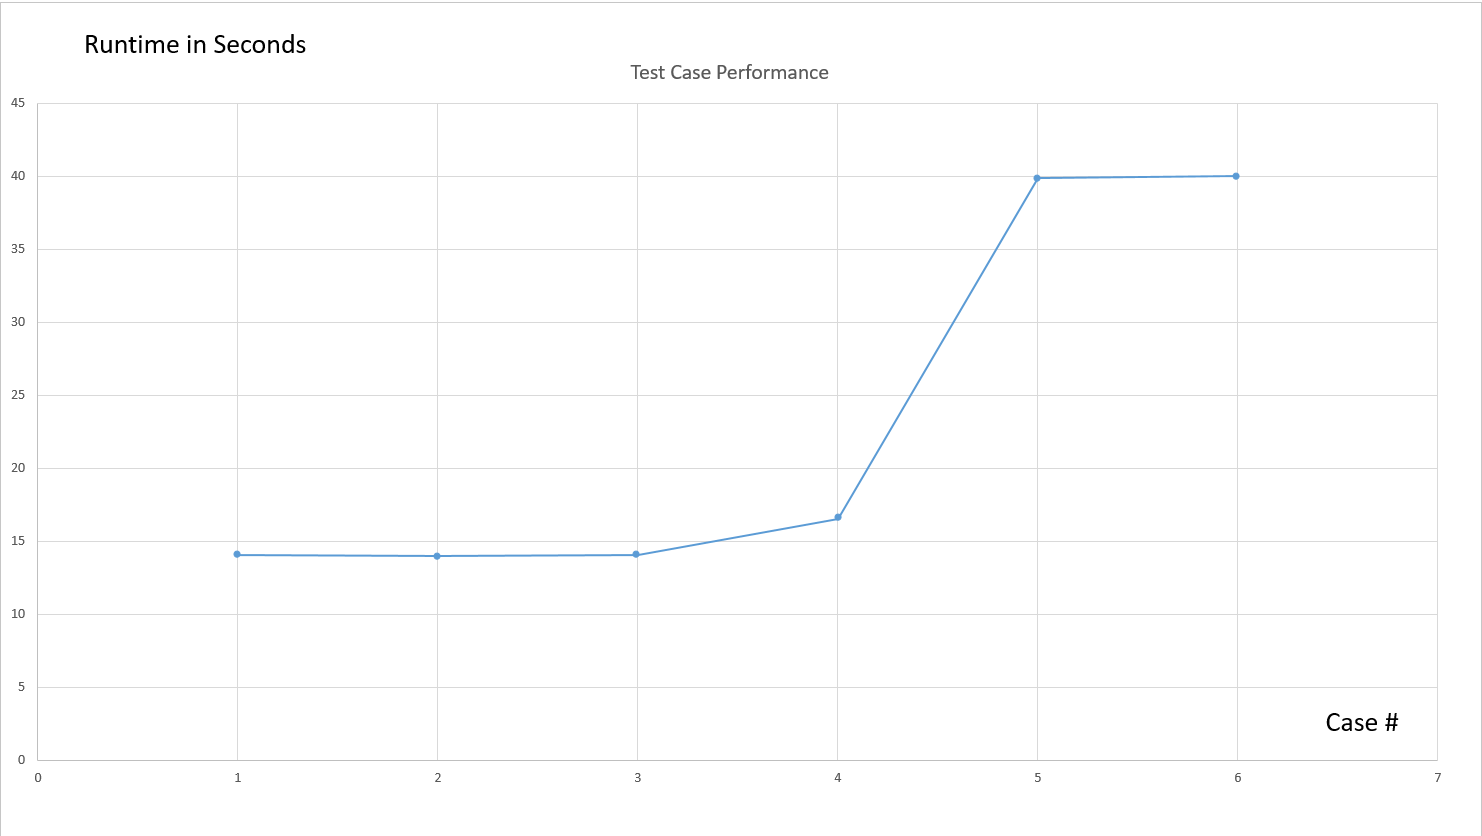
\includegraphics[width=\linewidth]{performance-graph.PNG}
  \caption{Run time results from images in Section 4.1}
  \label{fig:graph}
\end{figure}

\section{Future Improvements}
The performance results shows that the weak spots are shadows, specular highlights, and large number of objects. While the majority of these features are expected to significantly impact performance, my multithreading implementation could be enhanced to increase the performance of these features.

By using multiple threads to calculate shadows and trace multiply rays at a time, the exponential growth of the rendering equation can be combated. Other improvements that could be added are increased detail for light calculations, anti-aliasing, implementation of textures, and a module to load .obj files. 
\end{document}